%==============================================================================
%  LAB REPORT 1 — Basic Operations Using GPIO: Blinking LEDs
%  Compile with pdfLaTeX (works out of the box on Overleaf).
%
%  >>> PASTE YOUR GOOGLE DRIVE LINKS IN THE MACROS MARKED "EDIT ME" BELOW <<<
%==============================================================================
\documentclass[10pt,a4paper]{article}

%---------------------------------------- page geometry
\usepackage[a4paper,top=2.2cm,bottom=2.0cm,left=2.1cm,right=2.1cm,
            headsep=13pt,footskip=22pt]{geometry}

%---------------------------------------- encoding & fonts
\usepackage[T1]{fontenc}
\usepackage[utf8]{inputenc}
\usepackage{newtxtext,newtxmath}     % Times-like professional text + math
\usepackage[scaled=0.86]{beramono}   % clean monospace for code
\usepackage{microtype}

%---------------------------------------- graphics, colour, boxes
\usepackage{graphicx}
\usepackage[dvipsnames,table]{xcolor}
\usepackage{tikz}
\usepackage{circuitikz}
\usepackage[most]{tcolorbox}
\usepackage{booktabs}
\usepackage{array}
\usepackage{tabularx}
\usepackage{enumitem}
\usepackage{listings}
\usepackage{fancyhdr}
\usepackage{titlesec}
\usepackage{caption}
\usepackage{float}
\usepackage{needspace}
\usetikzlibrary{arrows.meta,positioning,calc,shadows.blur}
\ctikzset{bipoles/length=0.62cm}   % compact component symbols

%---------------------------------------- hyperlinks (load late)
\usepackage[hidelinks]{hyperref}
\usepackage{url}
% print a URL stored in a macro, safely (handles _ ~ % etc.)
\newcommand{\showurl}[1]{\expandafter\url\expandafter{#1}}

%==============================================================================
%  Student details
%==============================================================================
\newcommand{\studentname}{Chavan Atharva Sunil}
\newcommand{\rollnumber}{240003021}
\newcommand{\coursecode}{AA303 --- IoT for Space Applications}
\newcommand{\expdate}{6 August 2026}

%  Google Drive folder holding the demonstration videos and the source code
\urldef{\drivefolder}\url{https://drive.google.com/drive/folders/1T0wegsZBgEGQ7PwirSbTVWgo-MvS_5ov?usp=sharing}

%==============================================================================
%  Colour palette
%==============================================================================
\definecolor{ink}{HTML}{1B2733}      % body text / headings
\definecolor{accent}{HTML}{0B5FA5}   % primary blue
\definecolor{accentlt}{HTML}{E8F1FA} % pale blue fill
\definecolor{amber}{HTML}{C8791A}    % LED amber
\definecolor{amberlt}{HTML}{FDF3E3}
\definecolor{rule}{HTML}{C9D4DE}
\definecolor{soft}{HTML}{F5F7F9}
\definecolor{codebg}{HTML}{F7F9FB}
\definecolor{cmnt}{HTML}{6C8090}
\definecolor{kw}{HTML}{0B5FA5}
\definecolor{str}{HTML}{1C7C54}
\definecolor{num}{HTML}{9B2D5E}

\color{ink}

%==============================================================================
%  Headings
%==============================================================================
\titleformat{\section}
  {\normalfont\large\bfseries\color{accent}}
  {\raisebox{0pt}{\colorbox{accent}{\color{white}\bfseries\;\thesection\;}}}
  {0.7em}{}[\vspace{2pt}{\color{rule}\titlerule[0.8pt]}]
\titlespacing*{\section}{0pt}{14pt}{8pt}

\titleformat{\subsection}
  {\normalfont\normalsize\bfseries\color{ink}}{\thesubsection}{0.6em}{}
\titlespacing*{\subsection}{0pt}{11pt}{4pt}

\titleformat{\subsubsection}
  {\normalfont\small\bfseries\color{accent}}{}{0em}{}
\titlespacing*{\subsubsection}{0pt}{9pt}{2pt}

%==============================================================================
%  Header / footer
%==============================================================================
\pagestyle{fancy}
\fancyhf{}
\renewcommand{\headrulewidth}{0.4pt}
\renewcommand{\footrulewidth}{0pt}
\fancyhead[L]{\footnotesize\color{cmnt}\textsc{Lab Report 1} \,\textbar\, GPIO: Blinking LEDs}
\fancyhead[R]{\footnotesize\color{cmnt}\studentname\ \,\textbar\, \rollnumber}
\fancyfoot[C]{\footnotesize\color{cmnt}\thepage}

%==============================================================================
%  Captions & lists
%==============================================================================
\captionsetup{font=small,labelfont={bf,color=accent},skip=6pt}
\setlist[itemize]{leftmargin=1.35em,itemsep=2pt,topsep=3pt}
\setlist[enumerate]{leftmargin=1.6em,itemsep=2.5pt,topsep=3pt}
\renewcommand{\arraystretch}{1.18}

%==============================================================================
%  Custom boxes
%==============================================================================
\newtcolorbox{keybox}[1][]{
  enhanced, breakable, colback=accentlt, colframe=accent,
  boxrule=0pt, leftrule=3pt, arc=2pt, left=10pt, right=10pt, top=8pt, bottom=8pt,
  fontupper=\normalsize, #1}

\newtcolorbox{notebox}[1][]{
  enhanced, breakable, colback=amberlt, colframe=amber,
  boxrule=0pt, leftrule=3pt, arc=2pt, left=10pt, right=10pt, top=7pt, bottom=7pt,
  fontupper=\small, #1}

\newtcolorbox{titledbox}[2][]{
  enhanced, breakable, colback=white, colframe=rule, boxrule=0.6pt, arc=3pt,
  left=10pt, right=10pt, top=8pt, bottom=8pt,
  title={\bfseries\small #2}, coltitle=white, colbacktitle=accent,
  attach boxed title to top left={xshift=8pt,yshift=-8pt},
  boxed title style={boxrule=0pt,arc=2pt,left=6pt,right=6pt,top=2pt,bottom=2pt},
  #1}

%==============================================================================
%  Code listing style
%==============================================================================
\lstdefinestyle{prostyle}{
  backgroundcolor=\color{codebg},
  basicstyle=\ttfamily\scriptsize\color{ink},
  keywordstyle=\color{kw}\bfseries,
  commentstyle=\color{cmnt}\itshape,
  stringstyle=\color{str},
  numberstyle=\ttfamily\tiny\color{cmnt},
  numbers=left, numbersep=9pt, xleftmargin=17pt, xrightmargin=2pt,
  frame=single, framesep=6pt, rulecolor=\color{rule},
  breaklines=true, showstringspaces=false, tabsize=2,
  columns=fullflexible, keepspaces=true,
  aboveskip=8pt, belowskip=6pt,
  emphstyle=\color{num}\bfseries
}
\lstset{style=prostyle}

%==============================================================================
%  Reusable schematic macro
%  \gpioschematic{Board name}{p1}{p2}{p3}{p4}
%==============================================================================
\newcommand{\gpioschematic}[5]{%
\begin{circuitikz}[scale=0.86, transform shape, every node/.style={font=\footnotesize}]
  % ---- controller body
  \draw[fill=accentlt, draw=accent, line width=0.9pt, rounded corners=4pt]
        (-3.3,-0.15) rectangle (-0.6,4.9);
  \node[text=accent, font=\small\bfseries] at (-1.95,4.35) {#1};
  \node[text=cmnt,   font=\scriptsize]     at (-1.95,3.95) {GPIO header};

  % ---- pin pads + LED branches
  \foreach \y/\pin/\led in {3.15/#2/1, 2.2/#3/2, 1.25/#4/3, 0.3/#5/4}{
     \draw[fill=white, draw=accent, line width=0.6pt]
           (-0.92,\y-0.14) rectangle (-0.6,\y+0.14);
     \node[anchor=east, font=\scriptsize\bfseries, text=accent]
           at (-1.02,\y) {\pin};
     \draw[line width=0.7pt, accent] (-0.6,\y) -- (0.6,\y);
     \draw[line width=0.7pt] (0.6,\y) to[leD, l=LED\,\led] (3.6,\y);
     \draw[line width=0.7pt] (3.6,\y) -- (5.0,\y);
     \fill (5.0,\y) circle (1.3pt);
  }
  % ---- common ground rail
  \draw[line width=1pt] (5.0,0.3) -- (5.0,3.15);
  \draw[line width=1pt] (5.0,0.3) -- (5.0,-0.45);
  \node[ground] at (5.0,-0.45) {};
  \node[anchor=west, font=\scriptsize\bfseries] at (5.15,-0.3) {GND};
  \node[anchor=north, font=\scriptsize, text=cmnt, align=center]
        at (1.4,-0.95) {common ground rail on the breadboard, returned to the board's GND pin};
\end{circuitikz}}

% \gpioschematiceight{board}{p1}..{p8}   (p1 = MSB, p8 = LSB)
\newcommand{\gpioschematiceight}[9]{%
\begin{circuitikz}[scale=0.84, transform shape, every node/.style={font=\footnotesize}]
  \draw[fill=accentlt, draw=accent, line width=0.9pt, rounded corners=4pt]
        (-3.5,-0.15) rectangle (-0.6,8.05);
  \node[text=accent, font=\small\bfseries] at (-2.05,7.5) {#1};
  \node[text=cmnt,   font=\scriptsize]     at (-2.05,7.1) {GPIO header};
  \foreach \y/\pin/\bit/\wt in {%
      6.3/#2/7/128, 5.4/#3/6/64, 4.5/#4/5/32, 3.6/#5/4/16,
      2.7/#6/3/8,   1.8/#7/2/4,  0.9/#8/1/2,  0.0/#9/0/1}{
     \draw[fill=white, draw=accent, line width=0.6pt]
           (-0.92,\y-0.14) rectangle (-0.6,\y+0.14);
     \node[anchor=east, font=\scriptsize\bfseries, text=accent] at (-1.02,\y) {\pin};
     \draw[line width=0.7pt, accent] (-0.6,\y) -- (0.6,\y);
     \draw[line width=0.7pt] (0.6,\y) to[leD, l=LED\,\bit] (3.6,\y);
     \draw[line width=0.7pt] (3.6,\y) -- (5.0,\y);
     \fill (5.0,\y) circle (1.3pt);
     \node[anchor=west, font=\scriptsize, text=amber] at (5.25,\y) {bit \bit\ ($\wt$)};}
  \draw[line width=1pt] (5.0,0.0) -- (5.0,6.3);
  \draw[line width=1pt] (5.0,0.0) -- (5.0,-0.75);
  \node[ground] at (5.0,-0.75) {};
  \node[anchor=west, font=\scriptsize\bfseries] at (5.15,-0.6) {GND};
  \node[anchor=north, font=\scriptsize, text=cmnt, align=center]
        at (1.6,-1.25) {common ground rail on the breadboard, returned to the board's GND pin};
\end{circuitikz}}

%==============================================================================
\begin{document}

%------------------------------------------------------------------ TITLE BLOCK
\thispagestyle{empty}
\begin{tikzpicture}[remember picture, overlay]
  \fill[accent] (current page.north west) rectangle
        ($(current page.north east)+(0,-7.15cm)$);
  \fill[amber] ($(current page.north west)+(0,-7.15cm)$) rectangle
        ($(current page.north east)+(0,-7.3cm)$);
\end{tikzpicture}

\vspace*{0.35cm}
{\color{white}
 \noindent{\footnotesize\textsc{\coursecode}}\\[2pt]
 \noindent{\Large\bfseries Experiment 1 \,\textbar\, Lab Report}\\[8pt]
 \noindent{\huge\bfseries Basic Operations Using GPIO:}\\[6pt]
 \noindent{\huge\bfseries Blinking LEDs}\\[10pt]
 \noindent{\small Interfacing four LEDs with a Raspberry Pi and an ESP32}
}
\vspace{1.5cm}

\noindent
\begin{tabularx}{\textwidth}{@{}>{\bfseries\color{accent}}l X@{}}
\toprule
Submitted by  & \studentname \\
Roll Number   & \rollnumber \\
Date of Experiment & \expdate \\
Boards Used   & Raspberry Pi (BCM numbering) \quad\textbullet\quad ESP32 DevKit \\
\bottomrule
\end{tabularx}

\vspace{10pt}

%------------------------------------------------------------------ 1. AIM
\section{Aim}

\begin{keybox}
To understand the basic operation of GPIO (General Purpose Input/Output) pins by
interfacing LEDs with a \textbf{Raspberry Pi} and an \textbf{ESP32}. Four LEDs are
driven in two patterns --- all four blinking \textbf{simultaneously}, and a
\textbf{sequential} pattern with one LED ON at a time --- and the setup is then
extended to \textbf{eight LEDs} that display a decimal number, entered by the user at
the terminal or serial monitor, as its \textbf{8-bit binary} equivalent.
\end{keybox}

\subsection*{Objectives}
\begin{itemize}
  \item To identify the GPIO header of the Raspberry Pi and the ESP32 and select
        pins that are safe to use as general-purpose digital outputs.
  \item To configure the selected GPIO pins in \emph{output} mode from software and
        to wire four LEDs on a breadboard with a common ground return.
  \item To write, execute and verify blink programs in \textbf{Python}
        (\texttt{RPi.GPIO}) and in \textbf{C/C++} (Arduino core for ESP32).
  \item To display a user-entered decimal number ($0$--$255$) on eight LEDs by
        converting it to binary and mapping each bit to one GPIO pin.
  \item To observe and record the resulting output.
\end{itemize}

\subsection*{Brief Theory}
A GPIO pin is a pin on a microcontroller or single-board computer whose direction
and logic level are controlled entirely by software. When a pin is configured as a
digital output and written HIGH, the pin is internally connected to the supply rail
($3.3\,\mathrm{V}$ on both the Raspberry Pi and the ESP32); when written LOW it is
connected to ground. Connecting an LED between such a pin and GND therefore lets the
program switch the LED on and off.
Toggling the pin state in a loop, with a delay between transitions, produces a
visible blink; toggling four pins inside the same iteration makes all four LEDs
change state together.

\begin{notebox}
\textbf{Note on current limiting.} In this experiment the LEDs were connected
\emph{directly} to the GPIO pins, without series resistors, and the brief
demonstration ran without damage. Each GPIO pin can nevertheless source only a
limited current (about $16\,\mathrm{mA}$ on the Raspberry Pi and $12\,\mathrm{mA}$ on
the ESP32), and with a red LED whose forward drop is $\approx 2\,\mathrm{V}$ the
current is bounded only by the LED and the pin's own internal resistance. For
sustained use a series resistor of roughly $220\,\Omega$ per LED --- giving
$(3.3-2)/220 \approx 6\,\mathrm{mA}$ --- is the recommended practice.
\end{notebox}

%------------------------------------------------------------------ 2. MATERIALS
\Needspace{8\baselineskip}
\section{Materials Required}

\noindent
\begin{tabularx}{\textwidth}{@{}p{0.4cm} >{\raggedright\arraybackslash}p{5.2cm} c X@{}}
\toprule
\rowcolor{soft}
\multicolumn{1}{@{}l}{\textbf{\#}} & \textbf{Component} & \textbf{Qty.} & \textbf{Purpose in the setup} \\
\midrule
1 & Raspberry Pi (with SD card, OS installed) & 1 & Host board for Experiment 1 \\
2 & ESP32 development board                   & 1 & Host board for Experiment 2 \\
3 & Solderless breadboard                     & 1 & Mounting the LEDs and the ground rail \\
4 & LEDs (5\,mm, red)                         & 8 & Output indicators; 4 for the blink patterns, 8 for the binary display \\
5 & Male--female jumper wires                 & 16--20 & GPIO header to breadboard connections \\
6 & USB power supply / USB cable              & 1 & Powering and programming the board \\
7 & Computer (with Arduino IDE)               & 1 & Writing, compiling and uploading the code \\
\bottomrule
\end{tabularx}

\vspace{4pt}
\begin{notebox}
The Raspberry Pi was operated with a monitor, keyboard and mouse; the ESP32 was
programmed over USB from the Arduino IDE with the board set to
\texttt{ESP32 Dev Module}.
\end{notebox}

%============================================================ EXPERIMENT 1
\section{Methodology}

The experiment was carried out in two parts on two different platforms. In both
parts the electrical arrangement is identical --- only the pin numbers and the
programming environment differ.

\subsection{Experiment 1 --- Blinking Four LEDs Using Raspberry Pi GPIO}

Four LEDs were placed on the breadboard, each connected by a jumper wire
directly to a separate GPIO pin of the Raspberry Pi. The
cathodes of all four LEDs were tied to a common ground rail on the breadboard,
which was returned to a GND pin of the Pi.

All four GPIO pins were then configured as digital outputs in software. Inside an
infinite loop, the four pins were set HIGH at the same time --- turning all four
LEDs ON --- held for a fixed delay of one second, then set LOW at the same time,
turning all four LEDs OFF for another second. Repeating this cycle continuously
produces the blinking effect.

\subsubsection{GPIO connections}

\vspace{2pt}
\noindent
\begin{minipage}[t]{0.45\textwidth}
\vspace{0pt}
\begin{tabularx}{\linewidth}{@{}l l X@{}}
\toprule
\rowcolor{soft}
\textbf{LED} & \textbf{Raspberry Pi GPIO} & \textbf{Physical pin} \\
\midrule
LED 1 & GPIO 17 & Pin 11 \\
LED 2 & GPIO 18 & Pin 12 \\
LED 3 & GPIO 27 & Pin 13 \\
LED 4 & GPIO 22 & Pin 15 \\
\midrule
All cathodes & GND & Pin 6 / Pin 9 \\
\bottomrule
\end{tabularx}
\end{minipage}\hfill
\begin{minipage}[t]{0.52\textwidth}
\vspace{0pt}
\begin{titledbox}{Pin numbering}
\raggedright
The program uses \textbf{BCM} numbering (\texttt{GPIO.setmode(GPIO.BCM)}), i.e.\ the
Broadcom channel numbers printed in the pinout diagram, \emph{not} the physical
header positions. The physical pin column is given only for wiring convenience.
\end{titledbox}
\end{minipage}

\begin{figure}[htb]
\centering
\gpioschematic{Raspberry Pi}{GPIO 17}{GPIO 18}{GPIO 27}{GPIO 22}
\caption{Circuit schematic for Experiment 1. Each GPIO pin drives one LED directly;
all four cathodes return to the common GND rail on the breadboard.}
\label{fig:schematic-rpi}
\end{figure}

\subsubsection{Procedure}
\begin{enumerate}
  \item The four LEDs were placed on the breadboard, with the anode (longer leg) and
        cathode (shorter leg) of each LED in separate rows.
  \item The anode of each LED was taken by a jumper wire to a separate GPIO pin of
        the Raspberry Pi (GPIO 17, 18, 27 and 22); no series resistors were used.
        The wiring was checked with the board powered off.
  \item The cathodes of all four LEDs were connected to the common ground rail,
        which was wired back to a GND pin on the Pi.
  \item The four GPIO pins were configured as digital output pins in the Python
        program using \texttt{GPIO.setup()}.
  \item The program was executed on the Raspberry Pi.
  \item All four GPIO pins were set HIGH simultaneously, turning ON all four LEDs.
  \item After a fixed delay of one second, all four GPIO pins were set LOW
        simultaneously, turning OFF all four LEDs.
  \item The process was repeated continuously until the program was interrupted,
        after which \texttt{GPIO.cleanup()} released the pins.
\end{enumerate}

\subsubsection{Code (Python, \texttt{RPi.GPIO})}

\begin{lstlisting}[language=Python, caption={Blinking four LEDs simultaneously on the Raspberry Pi.}, label={lst:rpi}]
import RPi.GPIO as GPIO
import time

LED_PINS = [17, 18, 27, 22]      # BCM channel numbers

GPIO.setmode(GPIO.BCM)           # use Broadcom pin numbering
for pin in LED_PINS:             # configure every pin as a digital output
    GPIO.setup(pin, GPIO.OUT)

try:
    while True:
        # Turn all LEDs ON
        for pin in LED_PINS:
            GPIO.output(pin, GPIO.HIGH)
        time.sleep(1)

        # Turn all LEDs OFF
        for pin in LED_PINS:
            GPIO.output(pin, GPIO.LOW)
        time.sleep(1)

except KeyboardInterrupt:
    pass
finally:
    GPIO.cleanup()               # reset all pins to a safe state on exit
\end{lstlisting}

\subsubsection{Working}

All four LEDs are controlled together. When the GPIO pins are set HIGH, all four
LEDs turn ON; when the GPIO pins are set LOW, all four LEDs turn OFF. Because the
four \texttt{GPIO.output()} calls execute within microseconds of one another, the
transitions appear perfectly simultaneous to the eye.

\begin{figure}[H]
\centering
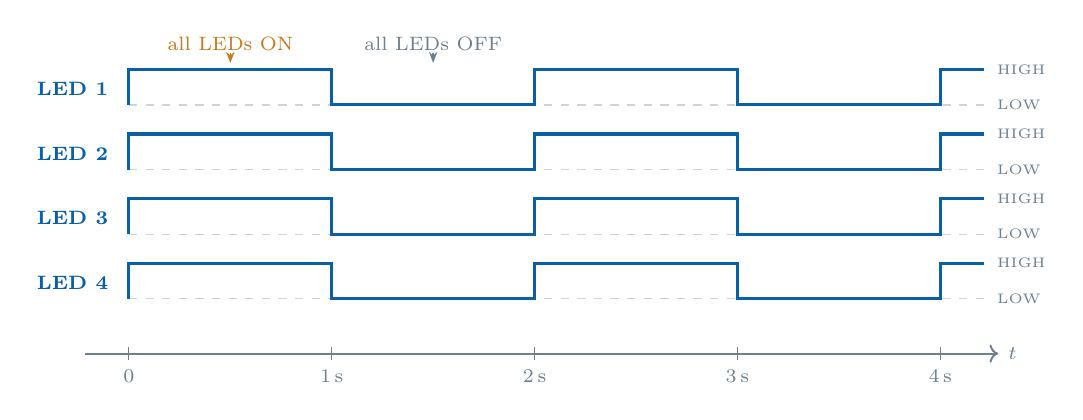
\begin{tikzpicture}[x=0.92cm, y=0.82cm]
  % time axis
  \draw[->, cmnt, line width=0.7pt] (0,-0.55) -- (12.6,-0.55)
        node[right, font=\scriptsize, text=cmnt] {$t$};
  \foreach \x/\lab in {0.6/0, 3.4/1\,s, 6.2/2\,s, 9.0/3\,s, 11.8/4\,s}{
      \draw[cmnt] (\x,-0.45) -- (\x,-0.65);
      \node[below, font=\scriptsize, text=cmnt] at (\x,-0.65) {\lab};}
  % four identical, in-phase waveforms
  \foreach \i/\y in {1/3.3, 2/2.3, 3/1.3, 4/0.3}{
    \node[anchor=east, font=\scriptsize\bfseries, text=accent] at (0.45,\y+0.25) {LED \i};
    \draw[rule, dashed, line width=0.4pt] (0.6,\y) -- (12.4,\y);
    \draw[accent, line width=1.1pt]
      (0.6,\y) -- (0.6,\y+0.55) -- (3.4,\y+0.55) -- (3.4,\y)
      -- (6.2,\y) -- (6.2,\y+0.55) -- (9.0,\y+0.55) -- (9.0,\y)
      -- (11.8,\y) -- (11.8,\y+0.55) -- (12.4,\y+0.55);
    \node[font=\tiny, text=cmnt, anchor=west] at (12.45,\y+0.55) {HIGH};
    \node[font=\tiny, text=cmnt, anchor=west] at (12.45,\y) {LOW};}
  % annotations
  \node[font=\scriptsize, text=amber] at (2.0,4.25) {all LEDs ON};
  \node[font=\scriptsize, text=cmnt]  at (4.8,4.25) {all LEDs OFF};
  \draw[amber, -{Stealth[length=4pt]}, line width=0.6pt] (2.0,4.1) -- (2.0,3.95);
  \draw[cmnt,  -{Stealth[length=4pt]}, line width=0.6pt] (4.8,4.1) -- (4.8,3.95);
\end{tikzpicture}
\caption{Timing diagram of the four GPIO outputs. The four waveforms are identical
and exactly in phase, which is what makes the LEDs blink simultaneously.}
\label{fig:timing}
\end{figure}


\begin{figure}[H]
\centering
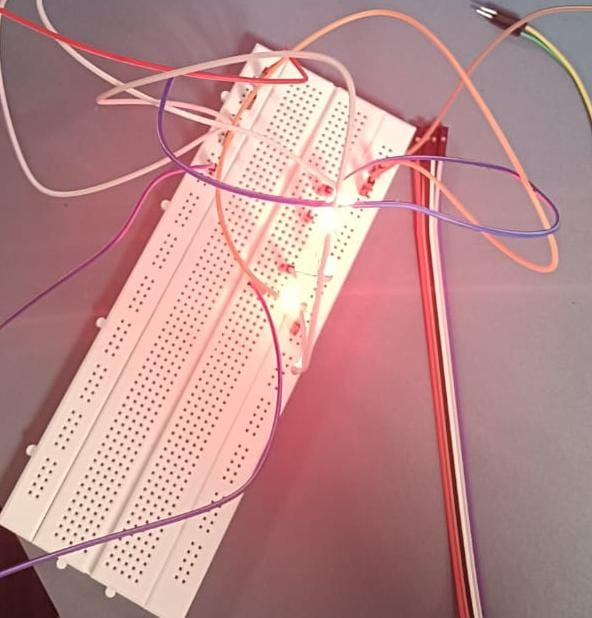
\includegraphics[width=0.46\textwidth, trim=40 198 0 40, clip]{figures/exp1_all_leds_on.jpg}
\caption{Experiment 1 --- all four LEDs lit simultaneously during the ON phase of the
blink cycle, with the jumper wires running to the GPIO header and all cathodes on the
common ground rail.}
\label{fig:photo-rpi}
\end{figure}

%============================================================ EXPERIMENT 2
\subsection{Experiment 2 --- Blinking Four LEDs Using ESP32}

The same four LEDs were re-wired to four GPIO pins of the ESP32 development board,
again connected directly, with all cathodes on the common ground rail returned to the
ESP32's GND pin.

The four GPIO pins were configured as digital outputs inside \texttt{setup()}.
Within \texttt{loop()}, all four pins were driven HIGH simultaneously to turn the
LEDs ON, held for one second using \texttt{delay(1000)}, then driven LOW
simultaneously to turn them OFF for another second. Since \texttt{loop()} is called
repeatedly by the Arduino core, the blinking continues indefinitely.

\subsubsection{Additional materials}
\begin{itemize}
  \item ESP32 development board, USB cable, and a computer with the Arduino IDE
        (ESP32 board support package installed).
\end{itemize}

\subsubsection{GPIO connections}

\vspace{2pt}
\noindent
\begin{minipage}[t]{0.45\textwidth}
\vspace{0pt}
\begin{tabularx}{\linewidth}{@{}l l X@{}}
\toprule
\rowcolor{soft}
\textbf{LED} & \textbf{ESP32 GPIO} & \textbf{Board label} \\
\midrule
LED 1 & GPIO 2  & D2  \\
LED 2 & GPIO 4  & D4  \\
LED 3 & GPIO 5  & D5  \\
LED 4 & GPIO 18 & D18 \\
\midrule
All cathodes & GND & GND \\
\bottomrule
\end{tabularx}
\end{minipage}\hfill
\begin{minipage}[t]{0.52\textwidth}
\vspace{0pt}
\begin{titledbox}{Choice of pins}
\raggedright
GPIO 2, 4, 5 and 18 are ordinary output-capable pins on the ESP32 and are free of
boot-strapping restrictions in this configuration. Input-only pins (GPIO 34--39)
cannot drive an LED and were therefore avoided.
\end{titledbox}
\end{minipage}

\begin{figure}[htb]
\centering
\gpioschematic{ESP32 DevKit}{GPIO 2}{GPIO 4}{GPIO 5}{GPIO 18}
\caption{Circuit schematic for Experiment 2. The topology is identical to
Figure~\ref{fig:schematic-rpi}; only the driving pins change.}
\label{fig:schematic-esp}
\end{figure}

\subsubsection{Procedure}
\begin{enumerate}
  \item The four LEDs were placed on the breadboard, anodes in separate rows.
  \item Each LED branch was connected to a separate GPIO pin of the ESP32
        (GPIO 2, 4, 5 and 18) and all cathodes were returned to the GND pin
        through the common ground rail.
  \item The ESP32 was connected to the computer over USB and the correct board and
        COM port were selected in the Arduino IDE.
  \item The program was written and uploaded, configuring all four GPIO pins as
        outputs in \texttt{setup()}.
  \item All four LEDs were switched ON simultaneously.
  \item After a one-second delay, all four LEDs were switched OFF simultaneously.
  \item The process repeated continuously as \texttt{loop()} re-executed.
\end{enumerate}

\subsubsection{Code (Arduino C++ for ESP32)}

\begin{lstlisting}[language=C++, caption={Blinking four LEDs simultaneously on the ESP32.}, label={lst:esp}]
int LED1 = 2;
int LED2 = 4;
int LED3 = 5;
int LED4 = 18;

void setup() {
  pinMode(LED1, OUTPUT);
  pinMode(LED2, OUTPUT);
  pinMode(LED3, OUTPUT);
  pinMode(LED4, OUTPUT);
}

void loop() {
  // Turn all LEDs ON
  digitalWrite(LED1, HIGH);
  digitalWrite(LED2, HIGH);
  digitalWrite(LED3, HIGH);
  digitalWrite(LED4, HIGH);
  delay(1000);

  // Turn all LEDs OFF
  digitalWrite(LED1, LOW);
  digitalWrite(LED2, LOW);
  digitalWrite(LED3, LOW);
  digitalWrite(LED4, LOW);
  delay(1000);
}
\end{lstlisting}

\subsubsection{Working}

The four LEDs operate simultaneously. When all four GPIO pins are HIGH, all four
LEDs turn ON; when all four GPIO pins are LOW, all four LEDs turn OFF. The behaviour
is identical to Figure~\ref{fig:timing}, confirming that the same GPIO concept
transfers unchanged from a Linux single-board computer to a microcontroller.

\subsection{Pattern 2 --- One LED ON at a Time}

After verifying the simultaneous blink, the same wiring was used for a
\textbf{sequential} pattern in which exactly one LED is lit at any instant. Only the
program changes: instead of writing the same level to all four pins, the loop walks
an index through the pin list, driving one pin HIGH while the other three are held
LOW, then advancing after a one-second delay. This produces a running-light
(``chaser'') effect across LED 1 $\to$ LED 2 $\to$ LED 3 $\to$ LED 4 and back to the
start.

\begin{figure}[H]
\centering
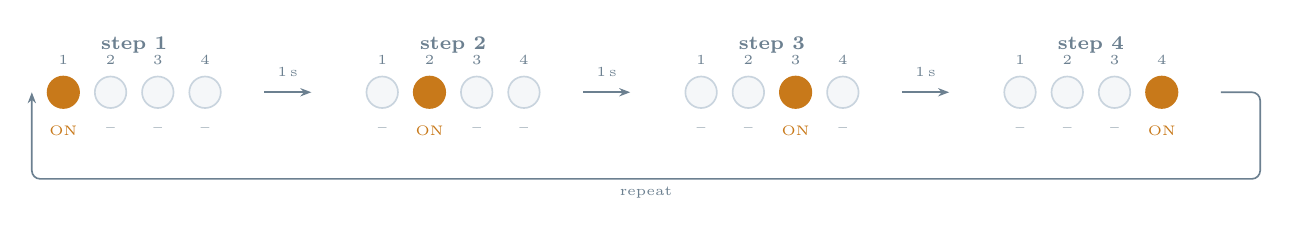
\begin{tikzpicture}[x=1cm, y=1cm]
  \foreach \step in {0,1,2,3}{
    \pgfmathsetmacro{\xo}{\step*4.05}
    \node[font=\scriptsize\bfseries, text=cmnt] at (\xo+1.5,1.15) {step \the\numexpr\step+1\relax};
    \foreach \i in {0,1,2,3}{
      \pgfmathsetmacro{\cx}{\xo+0.6+\i*0.6}
      \ifnum\i=\step
        \fill[amber] (\cx,0.55) circle (0.2);
        \draw[amber, line width=0.6pt] (\cx,0.55) circle (0.2);
        \node[font=\tiny, text=amber, anchor=north] at (\cx,0.25) {ON};
      \else
        \fill[soft] (\cx,0.55) circle (0.2);
        \draw[rule, line width=0.6pt] (\cx,0.55) circle (0.2);
        \node[font=\tiny, text=cmnt, anchor=north] at (\cx,0.25) {--};
      \fi
      \node[font=\tiny, text=cmnt, anchor=south] at (\cx,0.78) {\the\numexpr\i+1\relax};}
    \ifnum\step<3
      \draw[cmnt, -{Stealth[length=4pt]}, line width=0.6pt]
            (\xo+3.15,0.55) -- (\xo+3.75,0.55);
      \node[font=\tiny, text=cmnt, anchor=south] at (\xo+3.45,0.62) {1\,s};
    \fi}
  \draw[cmnt, -{Stealth[length=4pt]}, line width=0.6pt, rounded corners=3pt]
        (15.3,0.55) -- (15.8,0.55) -- (15.8,-0.55) -- (0.2,-0.55) -- (0.2,0.55);
  \node[font=\tiny, text=cmnt] at (8.0,-0.72) {repeat};
\end{tikzpicture}
\caption{The sequential pattern: exactly one LED is ON in each step, and the lit
position advances once per second before wrapping back to LED 1.}
\label{fig:sequence}
\end{figure}

\Needspace{9\baselineskip}
\begin{lstlisting}[language=Python, caption={Sequential pattern on the Raspberry Pi --- one LED ON at a time.}, label={lst:seq}]
while True:
    for on_pin in LED_PINS:                  # walk the lit position along the list
        for pin in LED_PINS:
            GPIO.output(pin, GPIO.HIGH if pin == on_pin else GPIO.LOW)
        time.sleep(1)
\end{lstlisting}

\noindent On the ESP32 the same logic was used inside \texttt{loop()}: the four
\texttt{digitalWrite()} calls set one pin HIGH and the remaining three LOW, followed
by \texttt{delay(1000)} before the lit position advances.

\subsection{Experiment 3 --- Eight-LED Binary Number Display}

In the final part of the experiment the setup was extended from four LEDs to
\textbf{eight}, and the LEDs were used not as a blinking pattern but as an
\textbf{8-bit output register}. The user types a decimal number in the range
$0$--$255$ --- on the Raspberry Pi at the terminal, on the ESP32 in the Arduino IDE
Serial Monitor --- and the program converts that number to its 8-bit binary form and
drives one LED per bit: a LED is ON where the bit is \texttt{1} and OFF where it is
\texttt{0}. The row of eight LEDs therefore reads directly as the binary value of the
number entered.

\subsubsection{GPIO connections}

\vspace{2pt}
\noindent
\begin{minipage}[t]{0.48\textwidth}
\vspace{0pt}
\begin{tabularx}{\linewidth}{@{}l l X@{}}
\toprule
\rowcolor{soft}
\textbf{Bit (weight)} & \textbf{Raspberry Pi} & \textbf{ESP32} \\
\midrule
bit 7 (128) & Pin 40 & GPIO 23 \\
bit 6 (64)  & Pin 38 & GPIO 22 \\
bit 5 (32)  & Pin 36 & GPIO 21 \\
bit 4 (16)  & Pin 35 & GPIO 19 \\
bit 3 (8)   & Pin 33 & GPIO 18 \\
bit 2 (4)   & Pin 32 & GPIO 5  \\
bit 1 (2)   & Pin 31 & GPIO 4  \\
bit 0 (1)   & Pin 29 & GPIO 2  \\
\midrule
All cathodes & GND & GND \\
\bottomrule
\end{tabularx}
\end{minipage}\hfill
\begin{minipage}[t]{0.49\textwidth}
\vspace{0pt}
\begin{titledbox}{Numbering used here}
\raggedright
The Raspberry Pi program for this part uses \textbf{BOARD} numbering
(\texttt{GPIO.setmode(GPIO.BOARD)}), so the numbers in the table are the
\emph{physical} header positions rather than the BCM channels used in
Experiment~1. The ESP32 column gives GPIO numbers as before. The most significant
bit is wired at the top of the row so that the LEDs read left-to-right in the same
order as the printed binary string.
\end{titledbox}
\end{minipage}

\begin{figure}[htb]
\centering
\gpioschematiceight{Raspberry Pi}{Pin 40}{Pin 38}{Pin 36}{Pin 35}{Pin 33}{Pin 32}{Pin 31}{Pin 29}
\caption{Circuit schematic for Experiment 3. Eight LEDs are driven directly from eight
GPIO pins, one per bit, with all cathodes on the common ground rail. The ESP32 wiring
is identical, using GPIO 23, 22, 21, 19, 18, 5, 4 and 2 in place of the header pins.}
\label{fig:schematic-8bit}
\end{figure}

\subsubsection{Principle of operation}

Each LED is assigned a place value: the leftmost carries $2^{7}=128$ and the rightmost
$2^{0}=1$. A number is displayed by testing its bits one at a time and writing the
result to the matching pin, so the pattern of lit LEDs is the binary representation of
the number. For example, $200 = 128 + 64 + 8$, giving the bit pattern
\texttt{11001000}:

\begin{figure}[H]
\centering
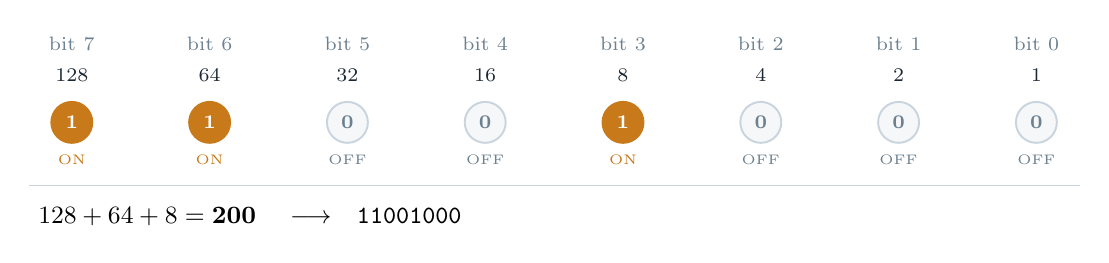
\begin{tikzpicture}[x=1cm, y=1cm]
  \foreach \i/\wt/\b in {0/128/1, 1/64/1, 2/32/0, 3/16/0, 4/8/1, 5/4/0, 6/2/0, 7/1/0}{
    \pgfmathsetmacro{\cx}{\i*1.75}
    \node[font=\scriptsize, text=cmnt] at (\cx,1.75) {bit \the\numexpr7-\i\relax};
    \node[font=\scriptsize\bfseries, text=ink] at (\cx,1.35) {$\wt$};
    \ifnum\b=1
      \fill[amber] (\cx,0.75) circle (0.26);
      \draw[amber, line width=0.7pt] (\cx,0.75) circle (0.26);
      \node[font=\scriptsize\bfseries, text=white] at (\cx,0.75) {1};
      \node[font=\tiny, text=amber] at (\cx,0.28) {ON};
    \else
      \fill[soft] (\cx,0.75) circle (0.26);
      \draw[rule, line width=0.7pt] (\cx,0.75) circle (0.26);
      \node[font=\scriptsize\bfseries, text=cmnt] at (\cx,0.75) {0};
      \node[font=\tiny, text=cmnt] at (\cx,0.28) {OFF};
    \fi}
  \draw[rule, line width=0.6pt] (-0.55,-0.05) -- (12.8,-0.05);
  \node[font=\small, anchor=west] at (-0.55,-0.45)
       {$128 + 64 + 8 = \mathbf{200}$ \quad$\longrightarrow$\quad
        \texttt{11001000}};
\end{tikzpicture}
\caption{Place values of the eight LEDs and the pattern displayed for the input
$200$. The same mapping was confirmed on the serial monitor for the inputs
$20 \rightarrow \texttt{00010100}$ and $25 \rightarrow \texttt{00011001}$.}
\label{fig:bits}
\end{figure}

\subsubsection{Procedure}
\begin{enumerate}
  \item Eight LEDs were placed in a row on the breadboard with all cathodes on the
        common ground rail, which was returned to the board's GND pin.
  \item Each anode was wired to its own GPIO pin in the order given in the table
        above, the most significant bit first.
  \item The program was run; it prompts for a decimal number on the terminal
        (Raspberry Pi) or on the Serial Monitor (ESP32).
  \item The entered number was converted to an 8-bit binary string, zero-padded on
        the left so that it always has exactly eight digits.
  \item Each bit was written to its corresponding GPIO pin, lighting the LEDs that
        correspond to the set bits.
  \item The binary string was also printed back to the console so that the display
        could be checked against the computed value.
  \item Steps 3--6 were repeated for several inputs, including $200$, $20$ and $25$.
\end{enumerate}

\Needspace{12\baselineskip}
\subsubsection{Code (Python, Raspberry Pi)}

\begin{lstlisting}[language=Python, caption={Displaying a decimal number on eight LEDs as 8-bit binary (Raspberry Pi).}, label={lst:bin-rpi}]
import RPi.GPIO as GPIO

# Physical (BOARD) pin numbers, most significant bit first
LED_PINS = [40, 38, 36, 35, 33, 32, 31, 29]

GPIO.setmode(GPIO.BOARD)
GPIO.setwarnings(False)
for pin in LED_PINS:
    GPIO.setup(pin, GPIO.OUT, initial=GPIO.LOW)

try:
    while True:
        number = int(input("Enter a number (0-255): "))
        if not 0 <= number <= 255:
            print("Out of range - please enter a value from 0 to 255.")
            continue

        bits = format(number, '08b')     # zero-padded to exactly 8 digits
        print(number, "->", bits)

        for pin, bit in zip(LED_PINS, bits):
            GPIO.output(pin, GPIO.HIGH if bit == '1' else GPIO.LOW)

except KeyboardInterrupt:
    print("\nExiting program")

finally:
    GPIO.cleanup()
\end{lstlisting}

\Needspace{12\baselineskip}
\subsubsection{Code (Arduino C++ for ESP32)}

\begin{lstlisting}[language=C++, caption={Displaying a decimal number on eight LEDs as 8-bit binary (ESP32).}, label={lst:bin-esp}]
const int LED_PINS[8] = {23, 22, 21, 19, 18, 5, 4, 2};  // MSB first

void setup() {
  Serial.begin(115200);
  for (int i = 0; i < 8; i++) {
    pinMode(LED_PINS[i], OUTPUT);
    digitalWrite(LED_PINS[i], LOW);
  }
  Serial.println("--- 8-Bit Binary LED Controller ---");
  Serial.println("Enter a number between 0 and 255.");
}

void loop() {
  if (Serial.available() > 0) {
    String line = Serial.readStringUntil('\n');
    line.trim();
    if (line.length() == 0) return;

    int number = line.toInt();
    if (number < 0 || number > 255) {
      Serial.println("Out of range - please enter a value from 0 to 255.");
      return;
    }

    Serial.print("Number: ");  Serial.print(number);
    Serial.print("  ->  Binary: ");

    for (int b = 7; b >= 0; b--) {
      int value = (number >> b) & 1;           // extract one bit
      digitalWrite(LED_PINS[7 - b], value);    // drive the matching LED
      Serial.print(value);
    }
    Serial.println();
  }
}
\end{lstlisting}

\subsubsection{Working}

Both programs perform the same three steps in a loop: read a decimal number, convert
it to a fixed-width 8-bit string, and write the eight bits to the eight GPIO pins.
The Python version uses \texttt{format(number, '08b')} and the ESP32 version shifts
and masks the number one bit at a time with \texttt{(number >> b) \& 1}; the two are
equivalent. Because the LEDs are wired most-significant-bit first, the illuminated
row matches the binary string printed on the console digit for digit.

\begin{figure}[htb]
\centering
\begin{minipage}[t]{0.485\textwidth}
\centering
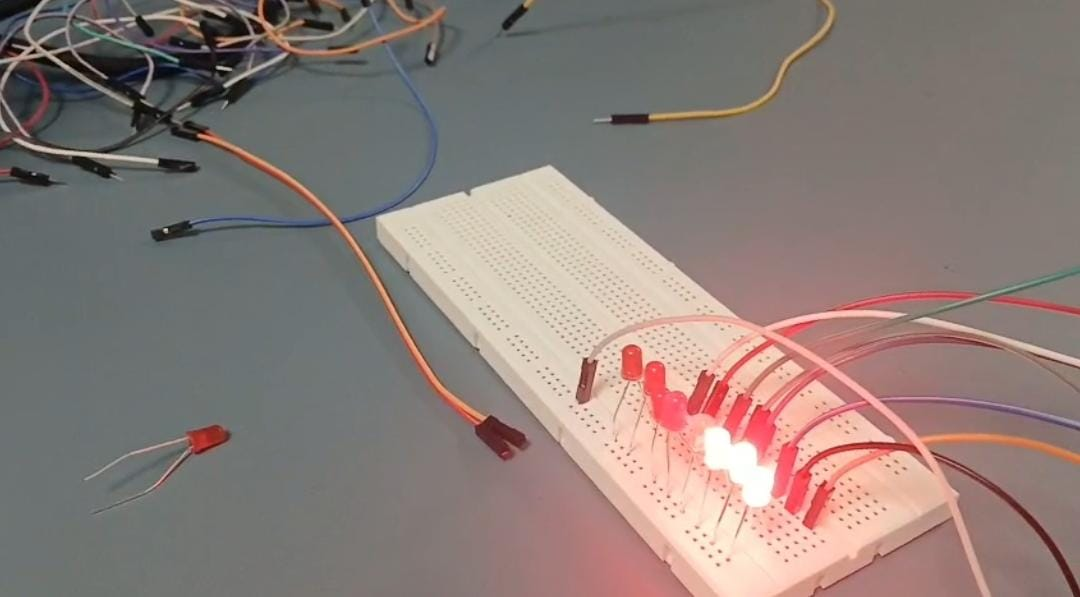
\includegraphics[width=\linewidth]{figures/rpi_8led_setup.jpg}
\end{minipage}\hfill
\begin{minipage}[t]{0.485\textwidth}
\centering
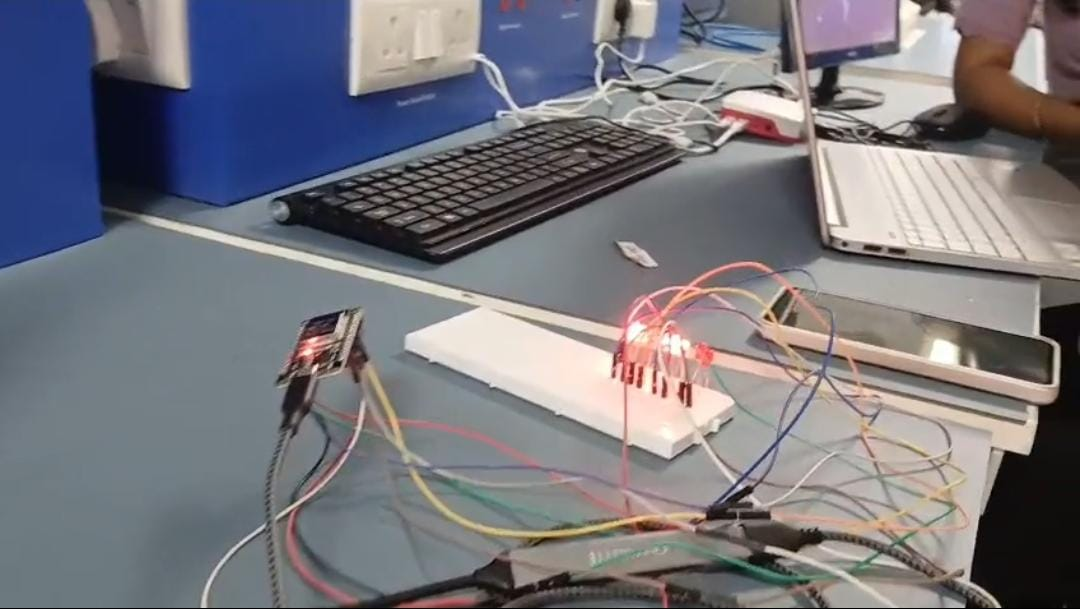
\includegraphics[width=\linewidth]{figures/esp32_8led_setup.jpg}
\end{minipage}
\caption{The eight-LED setup. \emph{Left:} the row of eight LEDs on the breadboard
displaying a bit pattern. \emph{Right:} the complete bench arrangement, with the
ESP32 on the left and the eight LEDs wired to its GPIO pins.}
\label{fig:8led-setup}
\end{figure}

%------------------------------------------------------------------ RESULT
\section{Result and Output}

\begin{keybox}
All three parts worked as intended on \textbf{both} the Raspberry Pi and the ESP32.
The four LEDs blinked \textbf{simultaneously}, turning ON and OFF together at
one-second intervals; in the second pattern exactly \textbf{one LED was ON at a time},
the lit position advancing once per second; and the eight-LED array correctly
displayed every decimal number entered as its \textbf{8-bit binary} equivalent.
\end{keybox}

\subsection*{Observed output}

\vspace{2pt}
\noindent
\begin{tabularx}{\textwidth}{@{}l l l X@{}}
\toprule
\rowcolor{soft}
\textbf{Pattern} & \textbf{GPIO state} & \textbf{LED state} & \textbf{Duration / remark} \\
\midrule
Simultaneous & All pins HIGH & LED 1--4 ON  & held $1\,$s; all four glow together \\
             & All pins LOW  & LED 1--4 OFF & held $1\,$s; all four go dark together \\
\midrule
Sequential   & One pin HIGH  & one LED ON   & held $1\,$s, then the lit position
                                              advances 1\,$\to$\,2\,$\to$\,3\,$\to$\,4 \\
             & other three LOW & three LEDs OFF & both cycles repeat continuously \\
\midrule
Binary (8 LEDs) & input $200$ & \texttt{11001000} & LEDs for bits 7, 6 and 3 lit \\
                & input $20$  & \texttt{00010100} & LEDs for bits 4 and 2 lit \\
                & input $25$  & \texttt{00011001} & LEDs for bits 4, 3 and 0 lit \\
\bottomrule
\end{tabularx}

\vspace{8pt}
\noindent The measured blink period in the first pattern was $2\,$s ($1\,$s ON $+$
$1\,$s OFF), i.e.\ $0.5\,$Hz with a $50\,\%$ duty cycle; the sequential pattern
completed one full sweep of the four LEDs every $4\,$s. Both matched the delay values
written in the programs. In the binary display the lit pattern agreed with the binary
string printed on the console for every value tested, and the display updated
immediately on each new entry.

\subsection*{Photographic evidence}

\vspace{2pt}
\noindent
\begin{minipage}[t]{0.485\textwidth}
\centering
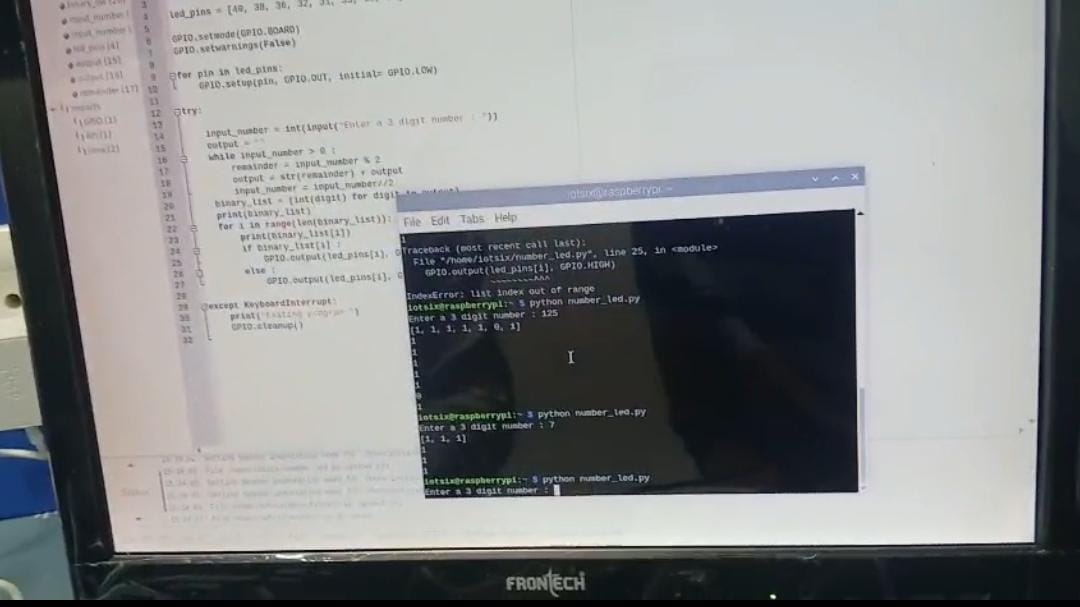
\includegraphics[width=\linewidth, trim=398 102 212 192, clip]{figures/rpi_terminal.jpg}
\captionof{figure}{The terminal session on the Raspberry Pi. The lower prompts read a
decimal input and print the resulting bit list; the traceback at the top is the
\texttt{IndexError} raised by the earlier, unpadded version of the program.}
\label{fig:rpi-terminal}
\end{minipage}\hfill
\begin{minipage}[t]{0.485\textwidth}
\centering
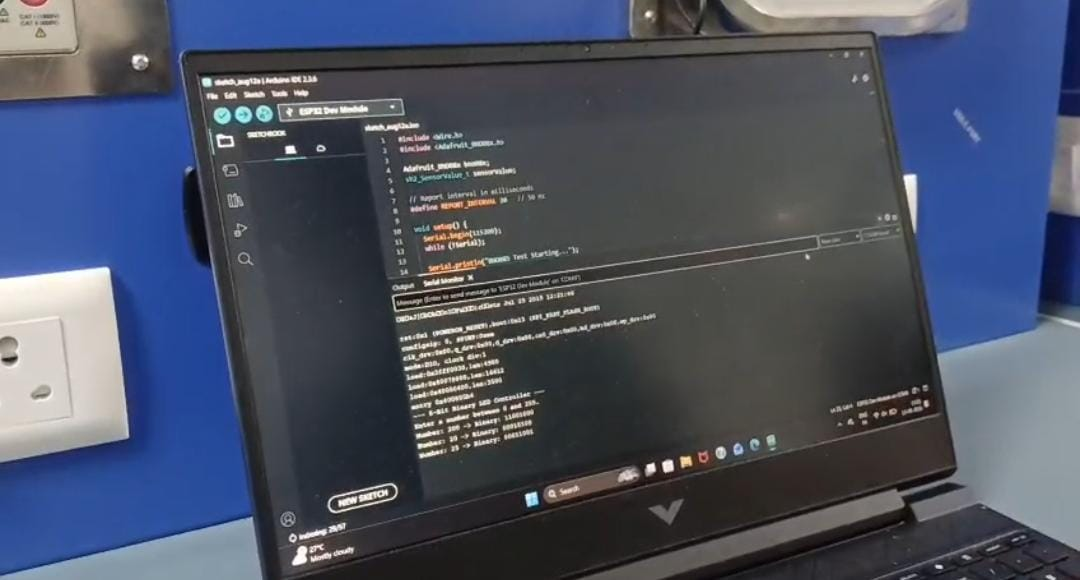
\includegraphics[width=\linewidth, trim=393 102 365 300, clip]{figures/esp32_serial_monitor.jpg}
\captionof{figure}{The Arduino IDE Serial Monitor for the ESP32, showing
$200 \rightarrow \texttt{11001000}$, $20 \rightarrow \texttt{00010100}$ and
$25 \rightarrow \texttt{00011001}$.}
\label{fig:esp-serial}
\end{minipage}

\vspace{10pt}

\noindent
\begin{minipage}[t]{0.485\textwidth}
\centering
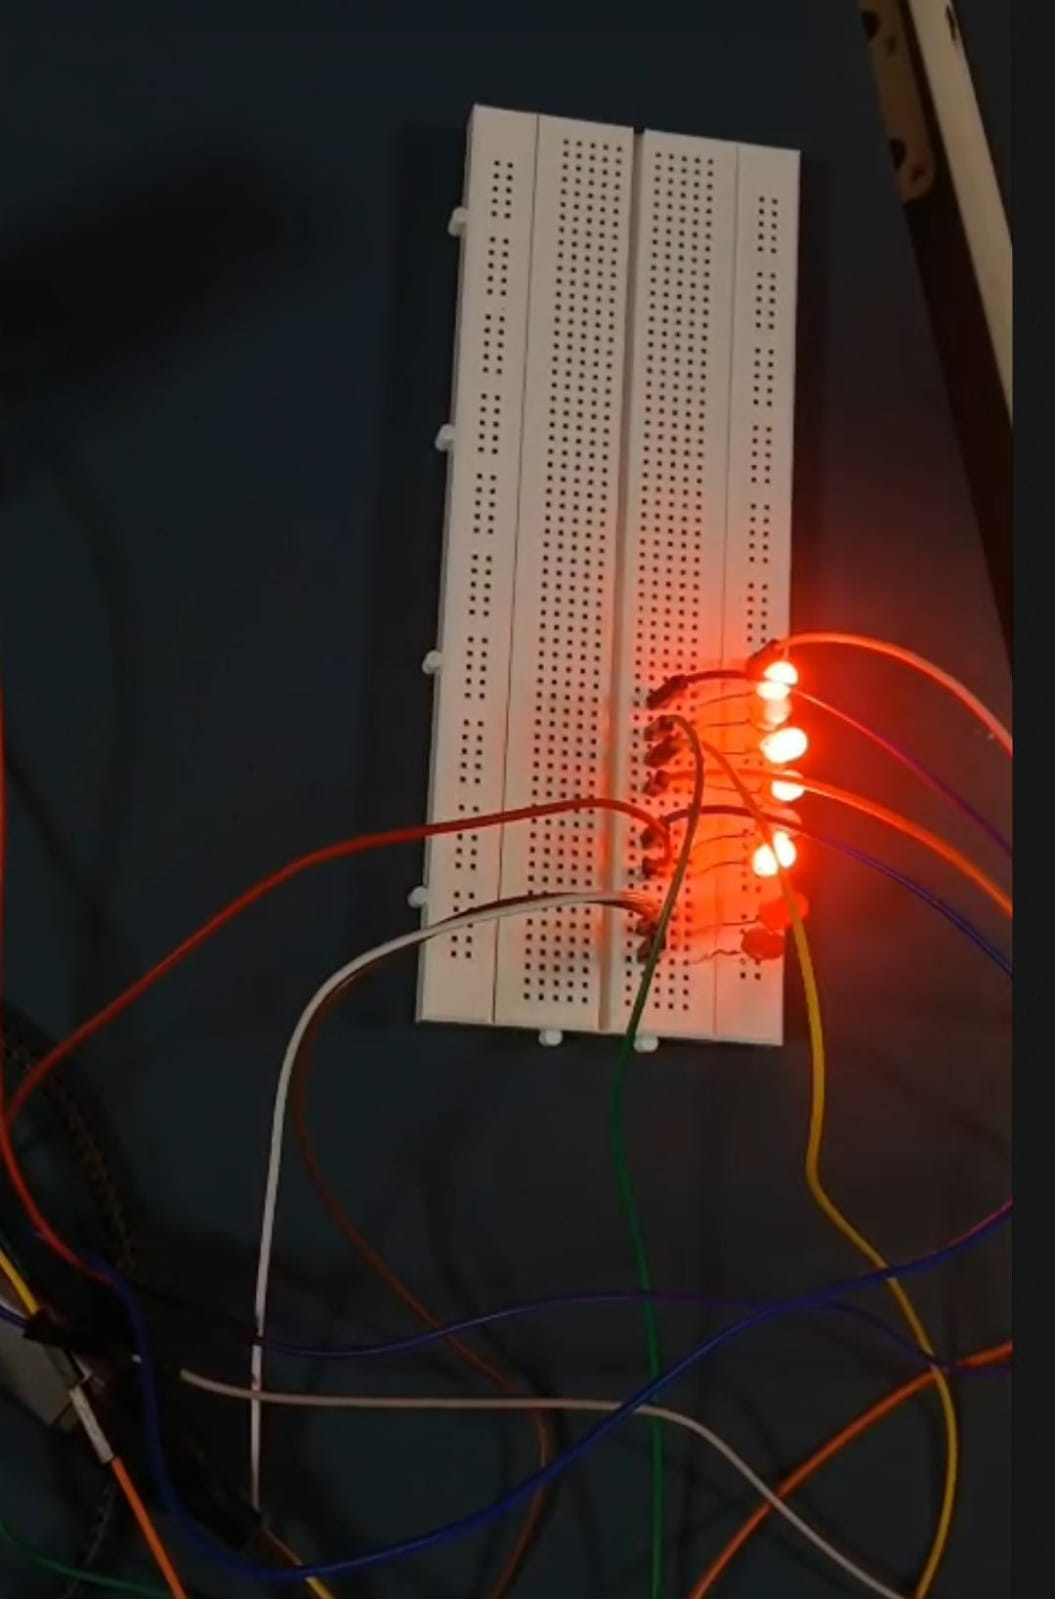
\includegraphics[width=\linewidth, trim=520 519 55 580, clip]{figures/binary_pattern_a.jpg}
\end{minipage}\hfill
\begin{minipage}[t]{0.485\textwidth}
\centering
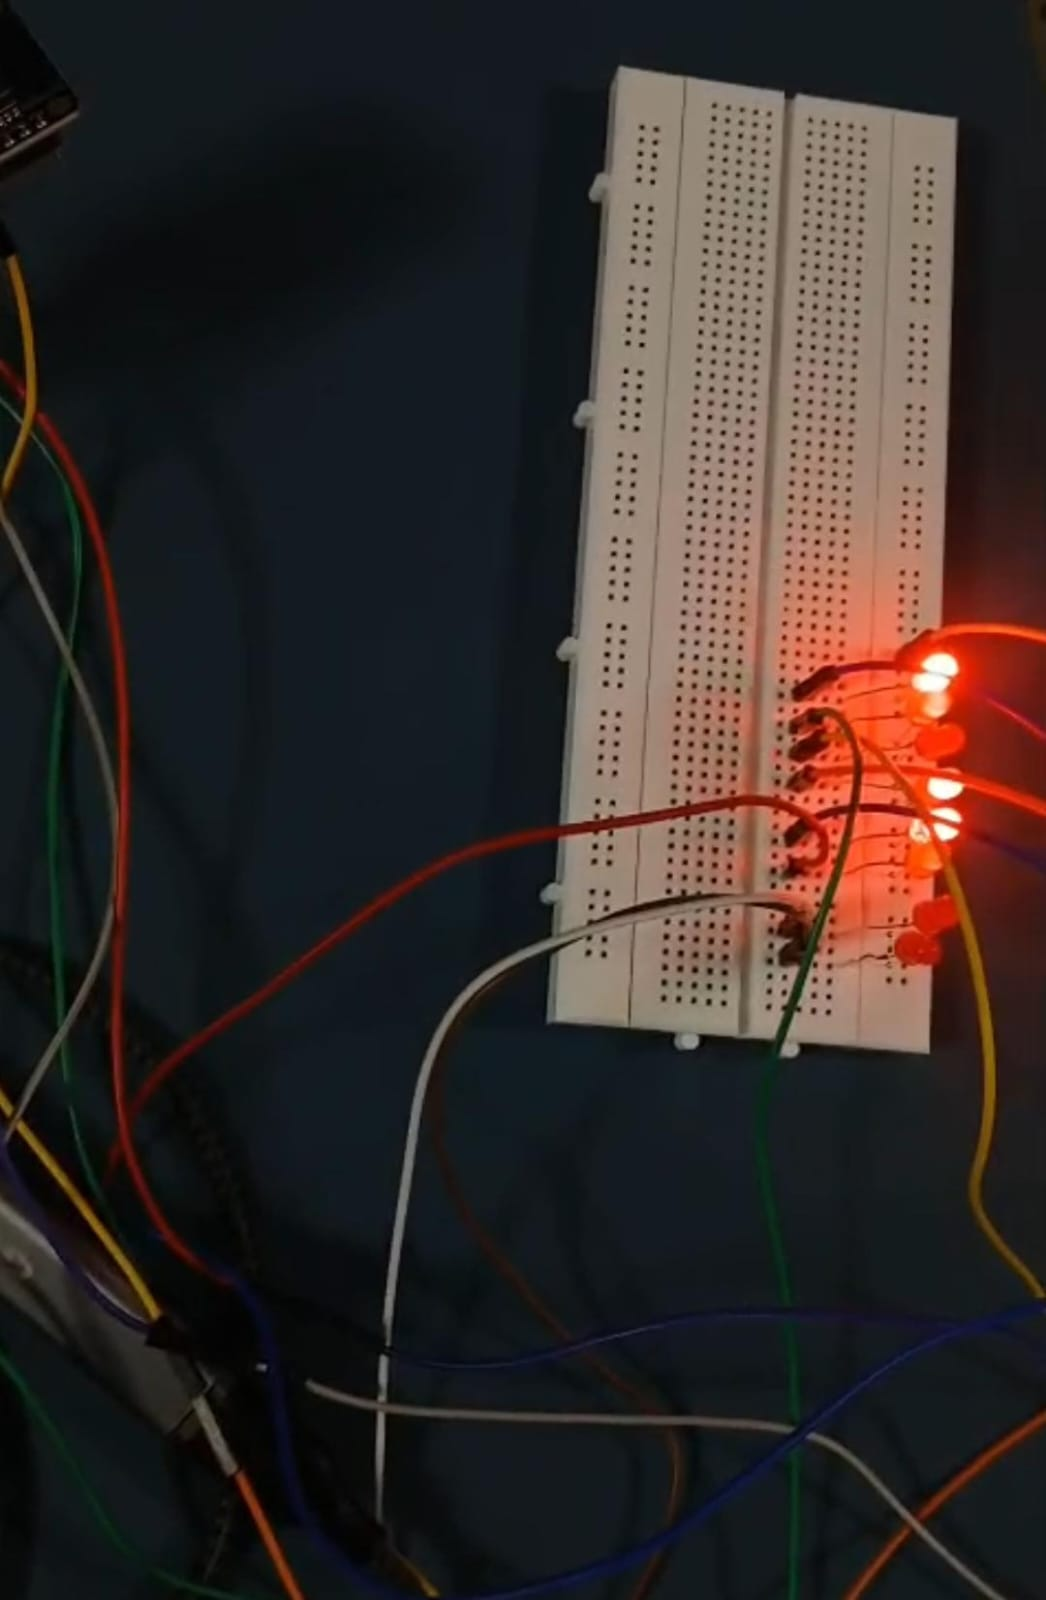
\includegraphics[width=\linewidth, trim=580 540 0 560, clip]{figures/binary_pattern_b.jpg}
\end{minipage}
\captionof{figure}{Two different numbers displayed on the eight-LED array; the lit
LEDs correspond to the set bits of the value entered on the console.}
\label{fig:patterns}

\vspace{10pt}

\subsection*{Video demonstration and code}

\begin{titledbox}[before skip=6pt]{Google Drive link}
\noindent The demonstration videos of all three parts on both boards, together with
this report and the complete source code for every listing above, are available in the
following shared folder:

\vspace{4pt}
\noindent\drivefolder

\vspace{4pt}
{\small\color{cmnt} Access has been set to \emph{anyone with the link can view}.}
\end{titledbox}

\vspace{6pt}

\subsection*{Discussion}
\begin{itemize}
  \item The LEDs switched in unison because all four output writes occur inside the
        same loop iteration; the few microseconds separating them are far below the
        threshold of visual perception.
  \item Reversing an LED (cathode to the GPIO pin) leaves it permanently dark, since
        the diode then blocks conduction --- a useful check when a single LED fails
        to light. Because no series resistors were used, the LEDs were driven close
        to the pin's current limit --- acceptable for a short demonstration, though a
        $220\,\Omega$ resistor per LED would be the safer arrangement.
  \item On the Raspberry Pi, \texttt{GPIO.cleanup()} in the \texttt{finally} block
        leaves no pin driven HIGH once the program is stopped.
  \item In the binary display the bit string \emph{must} be zero-padded to eight
        digits. An earlier version of the Raspberry Pi program built the bit list by
        repeated division, which yields only as many digits as the number needs, and
        indexing eight pins against that shorter list raised an
        \texttt{IndexError: list index out of range}. Using
        \texttt{format(number, '08b')} fixes this by always producing exactly eight
        characters.
  \item Wiring the most significant bit first means the row of LEDs can be read
        left-to-right in the same order as the printed binary string, which made
        checking the output against the console immediate.
\end{itemize}

%------------------------------------------------------------------ CONCLUSION
\section{Conclusion}

The experiment demonstrated the basic operation of GPIO pins as digital outputs: four
LEDs were interfaced with both the Raspberry Pi and the ESP32 and driven in two
patterns --- all four blinking together, and one LED lit at a time --- at one-second
intervals. The setup was then extended to eight LEDs used as an 8-bit output register,
displaying any decimal number from $0$ to $255$ entered at the terminal or serial
monitor as its binary equivalent.

The exercise established the complete path from software to hardware --- selecting
suitable pins, configuring them as outputs, wiring an external load to them, and
controlling that load in real time --- and, by producing identical
behaviour on two very different platforms, confirmed GPIO control as a
platform-independent foundation for the interfacing experiments that follow.

\end{document}
